\chapter{氢原子}\label{ch:b3:hydrogen-atom}

宇宙中九成的原子是氢：一个质子
束缚一个电子，是物理能够精确求解的唯一原子——
也是打开其他一切原子大门的钥匙。
\cref{ch:b3:hamiltonian-mechanics}中的旧量子论曾猜测它的能级；
如今，求解所需的工具已经齐备，能够\emph{导出}这些能级：库仑
势进入上一章的\omterm{prop:b3:schrodinger-three-dimensions:swave}{径向方程}，于是得到
能级 $-E_{\text{I}}/n^2$、\omterm{thm:b3:hydrogen-atom:levels}{玻尔半径}、化学元素周期表中的壳层
与支壳层，以及天文学家在每一团星云中读到的光谱线系。
同一解经过标度，
还可描述电离氦、μ 子原子、正电子素，以及
半导体中的电子–空穴“原子”；将\omterm{thm:b3:hydrogen-atom:levels}{主量子数}拉大到 $n
\approx 100$ 时，它描述半微米宽的里德伯原子，
其射电微弱信号可描绘银河系中的电离云，
其相互作用如今也正驱动量子计算机。
% NOTE: full radial solutions (Laguerre) admitted; ground state solved
% exactly; emphasis on scaling laws and applications.

\section{库仑问题的求解}

\begin{theorem}[氢原子的能级]\label{thm:b3:hydrogen-atom:levels}
\index{氢原子}\index{主量子数}\index{玻尔半径}
对于 $V(r) = -e^2/4\pi\varepsilon_0 r$（记 $k = e^2/4\pi
\varepsilon_0$），束缚态可用 $(n, l, m)$ 标记，其中
\[
E_n = -\frac{E_{\text{I}}}{n^2} , \qquad
E_{\text{I}} = \frac{m_{\text{e}}k^2}{2\hbar^2} = \qty{13.6}{eV} ,
\qquad n = 1, 2, 3, \dots
\]
对每个 $n$，\omterm{prop:b3:quantum-angular-momentum:harmonics}{轨道量子数} $l = 0, 1, \dots, n-1$ 以及
$m = -l, \dots, l$。自然长度为\omterm{thm:b3:hydrogen-atom:levels}{玻尔半径} $a_0 =
\hbar^2/m_{\text{e}}k = \qty{52.9}{pm}$；基态为
\[
\psi_{100} = \frac{1}{\sqrt{\pi a_0^3}}\;\eu^{-r/a_0} .
\]
能量\emph{仅}依赖于 $n$：计入 $m$ 与
$l$ 的取值，能级 $n$ 有 $n^2$ 重简并（计入自旋后加倍，
见\cref{ch:b3:spin-two-level}）——远多于各向同性所解释的
$(2l+1)$ 重简并。
\end{theorem}

\begin{proof}[部分证明]
对于基态，取 $u = Cr\,\eu^{-r/a}$，代入
$l = 0$ 的\omterm{prop:b3:schrodinger-three-dimensions:swave}{径向方程}：$u'' = (1/a^2 - 2/ar)u$，故
$-\tfrac{\hbar^2}{2m_{\text{e}}}u'' - \tfrac kr u = Eu$ 要求
$\hbar^2/m_{\text{e}}a = k$（与 $1/r$ 项匹配）——即
$a = a_0$，并且 $E = -\hbar^2/2m_{\text{e}}a_0^2 = -E_{\text{I}}$。
一般解（拉盖尔多项式，$n - l - 1$ 个径向
节点）在此承认；构造的每一步都是初等的，但
过程冗长。“偶然”的 $l$ 简并反映了纯 $1/r$ 力的
一个经典秘密——开普勒椭圆不进动，并且
存在一个额外的守恒矢量（拉普拉斯–龙格–楞次矢量）沿固定的
长轴方向；其量子版本正是把不同 $l$ 联系到
同一能量的原因（见\cref{exo:b3:hydrogen-atom:12}）。
\end{proof}

\begin{omfigure}
\begin{tikzpicture}[font=\small, >=Stealth]
  % energy scale: E = -13.6/n^2, map E -> y = 5.6 + E*0.42 (E in eV)
  % n=1: y=-0.11? choose y(E) = 5.9 + 0.42*E: n1: 0.19, n2: 4.47, n3: 5.27, n4: 5.55, inf: 5.9
  \draw[->] (-0.4,-0.4) -- (-0.4,6.6);
  \node[anchor=south] at (-0.4,6.6) {$E$（eV）};
  % continuum
  \fill[gray!15] (0,5.9) rectangle (8.6,6.45);
  \node[anchor=west, font=\footnotesize] at (8.7,6.15) {连续谱：电离};
  \draw[thick] (0,5.9) -- (8.6,5.9);
  \node[anchor=east, font=\footnotesize] at (-0.5,5.9) {$0$};
  % levels, split by l columns
  \foreach \n/\y in {1/0.19, 2/4.47, 3/5.27, 4/5.55}
    {\node[anchor=east, font=\footnotesize] at (-0.5,\y) {$-13.6/\n^2$};}
  % l columns: s at x 0-1.4, p at 1.9-3.3, d at 3.8-5.2, f 5.7-7.1
  \node[font=\footnotesize] at (0.7,-0.3) {$l = 0$ ($s$)};
  \node[font=\footnotesize] at (2.6,-0.3) {$l = 1$ ($p$)};
  \node[font=\footnotesize] at (4.5,-0.3) {$l = 2$ ($d$)};
  \node[font=\footnotesize] at (6.4,-0.3) {$l = 3$ ($f$)};
  \draw[very thick, omDef] (0,0.19) -- (1.4,0.19);
  \foreach \x in {0,1.9} \draw[very thick, omDef] (\x,4.47) -- ({\x+1.4},4.47);
  \foreach \x in {0,1.9,3.8} \draw[very thick, omDef] (\x,5.27) -- ({\x+1.4},5.27);
  \foreach \x in {0,1.9,3.8,5.7} \draw[very thick, omDef] (\x,5.55) -- ({\x+1.4},5.55);
  % series arrows
  \draw[->, omExo, thick] (0.5,4.47) -- (0.6,0.24);
  \draw[->, omExo, thick] (1.0,5.27) -- (0.85,0.24);
  \node[omExo, font=\footnotesize, anchor=west] at (0.95,2.3) {莱曼系（紫外）};
  \draw[->, omThm, thick] (2.6,5.27) -- (2.45,4.52);
  \draw[->, omThm, thick] (3.1,5.55) -- (2.9,4.52);
  \node[omThm, font=\footnotesize, anchor=west] at (3.25,4.95) {巴耳末系（可见）};
  \node at (1.9,1.55) {};
\end{tikzpicture}

{\small 氢原子能级 $-E_{\text{I}}/n^2$，按 $l$ 展开：
同一 $n$ 的所有支壳层重合（库仑“偶然”简并）。向下跃迁
终止于 $n = 1$ 者构成紫外的莱曼系；终止于 $n = 2$ 者构成
可见光的巴耳末系，
它使星云呈红色。}
\end{omfigure}

\section{电子在何处}

\begin{proposition}[径向分布]\label{prop:b3:hydrogen-atom:radial}
\index{径向概率}
电子位于 $r$ 与 $r + \dd r$ 之间的概率
为 $P(r)\,\dd r$，其中 $P(r) = |u(r)|^2$，即
\cref{thm:b3:quantum-angular-momentum:radial}中归一化径向函数的平方。对于最低的几个态：
$P_{1s} \propto r^2\eu^{-2r/a_0}$，恰在 $r = a_0$ 处取峰值，
且 $\langle r\rangle = \tfrac32 a_0$；$P_{2s}$ 呈现两个
被球面\emph{节点}隔开的峰；$P_{2p} \propto
r^4\eu^{-r/a_0}$，在 $4a_0$ 处取峰值。一般地 $\langle r\rangle
\approx n^2a_0$：原子随激发\emph{平方}地增大，
而其束缚按 $1/n^2$ 减弱——这正是
\cref{pb:b3:hydrogen-atom:1}中里德伯巨星的依据。
\end{proposition}
\admitted

\begin{omfigure}
\begin{tikzpicture}
  \begin{axis}[omaxis, axis x line=bottom, axis y line=left,
    width=11.6cm, height=5.8cm, xmin=0, xmax=14, ymin=0, ymax=0.62,
    xlabel={$r/a_0$}, ylabel={$P(r)$（每 $a_0$）},
    xlabel style={at={(axis description cs:0.5,-0.1)}, anchor=north},
    xtick={1,4,5,10}, ytick=\empty, clip=false,
    legend style={font=\scriptsize, at={(0.95,0.9)}, anchor=north east,
      draw=none, fill=none}]
    \addplot[omDef, very thick, domain=0:8, samples=120] {4*x*x*exp(-2*x)};
    \addlegendentry{$1s$}
    \addplot[omThm, thick, domain=0:14, samples=140] {0.125*x*x*(2-x)^2*exp(-x)};
    \addlegendentry{$2s$}
    \addplot[omExo, thick, domain=0:14, samples=140] {x^4*exp(-x)/24};
    \addlegendentry{$2p$}
    \draw[gray, dashed] (axis cs:1,0) -- (axis cs:1,0.545);
  \end{axis}
\end{tikzpicture}

{\small \omterm{prop:b3:hydrogen-atom:radial}{径向概率}密度。$1s$ 态的峰恰好位于
$a_0$ 处；$2s$ 态带有一个球面节点，以及一个靠近原子核的瓣——
即将决定元素周期表次序的“穿透”效应，而
$2p$ 态受\omterm{thm:b3:quantum-angular-momentum:radial}{离心势垒}阻隔，
远离原子核。}
\end{omfigure}

\begin{example}[读取尺寸]\label{ex:b3:hydrogen-atom:sizes}
基态：直径 \qty{0.1}{nm}，束缚能 \qty{13.6}{eV}，
正是全部化学的尺度。当 $n = 10$ 时：半径 $\sim\qty{5}{nm}$，
束缚能 \qty{0.136}{eV}，束缚松散。当 $n = 100$ 时：一个
\emph{微米}量级的原子，束缚能 \qty{1.4}{meV}，极弱的
场即可破坏它——然而星际空间足够空旷，
使这类原子得以存活并“广播”
（见\cref{pb:b3:hydrogen-atom:1}）。
\end{example}

\section{光谱}

\begin{proposition}[线系与选择定则]\label{prop:b3:hydrogen-atom:series}
\index{巴耳末线系}\index{赖曼线系}
一次 $n' \to n$ 的跃迁发出的波长为
\[
\frac{1}{\lambda} = R_{\text{H}}\Big(\frac{1}{n^2} -
\frac{1}{n'^2}\Big) , \qquad
R_{\text{H}} = \frac{E_{\text{I}}}{hc} = \qty{1.097e7}{m^{-1}} ,
\]
遵从偶极选择定则 $\Delta l = \pm1$（光子
携带 $\hbar$）。\omterm{prop:b3:hydrogen-atom:series}{赖曼线系}（$\to n = 1$）位于远
紫外区，始于 \qty{121.6}{nm}；\omterm{prop:b3:hydrogen-atom:series}{巴耳末线系}（$\to n = 2$）
始于红色的 $H\alpha$ 谱线 \qty{656.3}{nm}，正是发射星云与日珥的颜色；
帕邢线系及之后各线系移入红外区，
在 $n = 110$ 与 $109$ 之间，同一公式落在
\qty{5.0}{GHz} 处，氢原子从
紫外一直“说”到无线电波段。
\end{proposition}

\begin{proof}
由能量守恒，并结合\cref{thm:b3:hydrogen-atom:levels}；
$R_{\text{H}}$ 与\cref{pb:b3:hamiltonian-mechanics:1}中相同，此处
由推导得出，而非假设。
\end{proof}

\begin{example}[类氢原子：一个解，多种原子]\label{ex:b3:hydrogen-atom:scaling}
将质子的电荷换为 $Ze$，并把电子换为任意绕转的
质量 $\mu$：每个公式按下式重新标度：
\[
a \to a_0\,\frac{m_{\text{e}}}{\mu}\,\frac1Z , \qquad
E_{\text{I}} \to E_{\text{I}}\,\frac{\mu}{m_{\text{e}}}\,Z^2 .
\]
He$^+$（$Z = 2$）：\qty{54.4}{eV}。重原子的内层电子
（$Z \sim 30$）：K 壳层能量处于 keV 量级，即莫塞莱借以排列元素次序的
特征 X 射线
（见\cref{exo:b3:hydrogen-atom:5}）。μ 子氢（$\mu = 207
m_{\text{e}}$）：飞米量级的原子，直接探测质子本身。
正电子素（$e^+e^-$，$\mu = m_{\text{e}}/2$）：束缚能减半，
尺寸加倍，寿命短暂，最终以湮灭光子结束。
而在半导体中，电子与空穴
在屏蔽性电介质中，以较小的有效质量相互绕转：一个
\emph{激子}，即同一原子膨胀至十纳米、
束缚能降至毫电子伏量级（见\cref{exo:b3:hydrogen-atom:7}）——氢与其说是原子，
不如说是一个模板。
\end{example}

\begin{omfigure}
\begin{tikzpicture}[font=\small]
  % size comparison, hand-drawn
  \draw[omDef, thick, fill=omDef!12] (1.2,0) circle (1.05);
  \fill[omDef] (1.2,0) circle (1.5pt);
  \node[align=center, font=\footnotesize] at (1.2,-1.75)
    {氢 \\$a_0$，\qty{-13.6}{eV}};
  \draw[omThm, thick, fill=omThm!12] (4.6,0) circle (0.42);
  \fill[omThm] (4.6,0) circle (1.5pt);
  \node[align=center, font=\footnotesize] at (4.6,-1.75)
    {μ 子氢 \\$a_0/207$（此处为 $\times 40$）\\\qty{-2.5}{keV}};
  \draw[omExo, thick, fill=omExo!12] (8.1,0) circle (1.55);
  \fill[omExo] (8.1,0) circle (1.5pt);
  \node[align=center, font=\footnotesize] at (8.1,-2.25)
    {正电子素 \\$2a_0$，\qty{-6.8}{eV}};
  \draw[omProp, thick, fill=omProp!10] (12.4,0) circle (2.0);
  \fill[omProp] (12.4,0) circle (1.5pt);
  \node[align=center, font=\footnotesize] at (12.4,-2.75)
    {晶体中的激子 \\$\sim 170\,a_0$（此处为 $\div 50$）\\$\sim\qty{-7}{meV}$};
\end{tikzpicture}

{\small 一个解，四种“原子”：通过重标度质量、电荷与
介电环境，氢原子便成为探测质子的工具、
纯量子电动力学的检验，以及半导体中发光的
类原子。}
\end{omfigure}

\begin{method}[氢原子系统的处理]\label{met:b3:hydrogen-atom:method}
(1) 先做标度：$a \propto 1/\mu Z$，$E \propto \mu Z^2$，可将任意氢原子
结果化为任意类氢结果。(2) 尺寸：$\langle
r\rangle \sim n^2a$；能级 $n$ 附近的间距为 $\dd E/\dd n =
2E_{\text{I}}/n^3$。(3) 光谱：里德伯公式加 $\Delta l =
\pm1$。(4) 穿透：$s$ 态感受到原子核，高 $l$ 态则在核外运动——
这正是多电子化学的杠杆。(5)
可靠的锚点：$\qty{13.6}{eV}$、$\qty{52.9}{pm}$、
$\qty{121.6}{nm}$、$\qty{656.3}{nm}$——四个值得
终身牢记的数字。
\end{method}

\begin{omfigure}
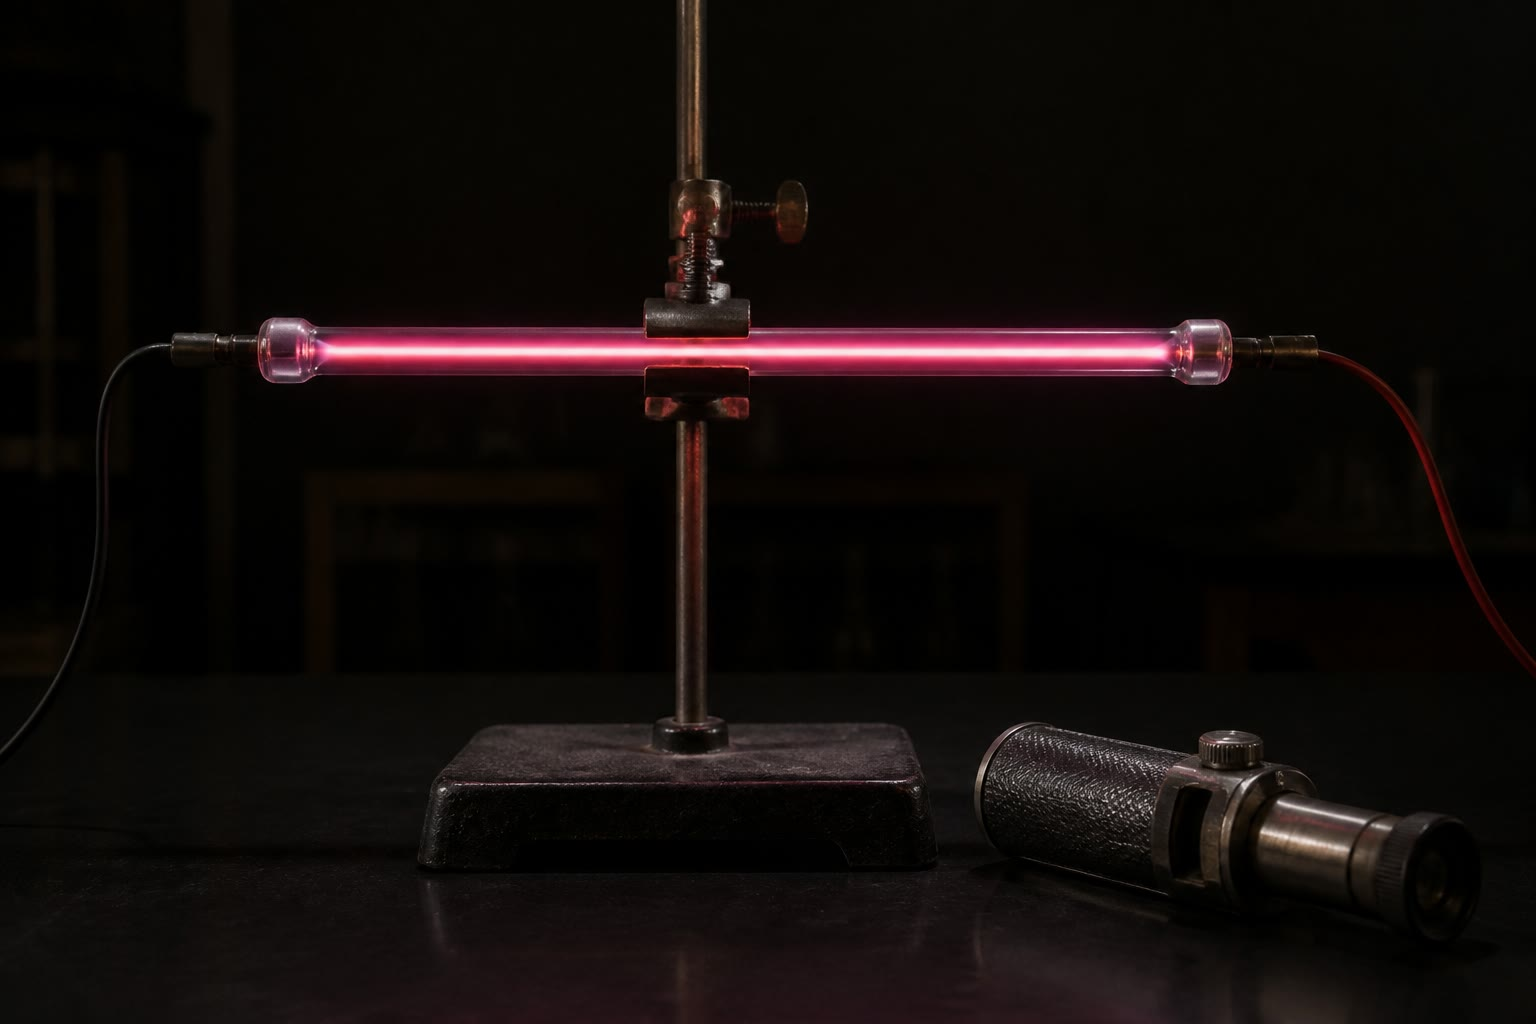
\includegraphics[width=0.58\linewidth]{images/book5/ai/b5-11-discharge-tube.jpg}

{\small 氢气放电管与袖珍分光镜：粉红色辉光分光后，变为巴耳末线——这是本章由库仑势导出的整数“指纹”。}
\end{omfigure}

\section{练习}

\begin{exercise}[$\star$]\label{exo:b3:hydrogen-atom:1}
(a) 代入验证 $u = Cr\eu^{-r/a_0}$ 满足 $l = 0$ 的\omterm{prop:b3:schrodinger-three-dimensions:swave}{径向方程}，
其中 $E = -E_{\text{I}}$，且 $a_0 =
\hbar^2/m_{\text{e}}k$。(b) 归一化它（$\int_0^\infty
x^2\eu^{-x}\dd x = 2$）。(c) 检查 $a_0$ 与
$E_{\text{I}}$ 的量纲。(d) 为什么不存在低于 $-E_{\text{I}}$ 的态
（可借助\cref{exo:b3:schrodinger-three-dimensions:12} 论证）？
\end{exercise}

\begin{exercise}[$\star$]\label{exo:b3:hydrogen-atom:2}
计算：(a) 莱曼 $\alpha$ 线与莱曼
极限的波长；(b) 巴耳末系前三条谱线及巴耳末
极限——哪些可见，颜色分别是什么？(c) 帕邢系的范围；
(d) $n = 110 \to 109$ 跃迁的频率。
\end{exercise}

\begin{exercise}[$\star$]\label{exo:b3:hydrogen-atom:3}
对基态：(a) 求 $P_{1s}(r)$ 的极大值位置；(b)
计算 $\langle r\rangle$；(c) 计算电子处于 $2a_0$ 之外的概率
（$\int_x^\infty t^2\eu^{-t}\dd t = (x^2 +
2x + 2)\eu^{-x}$）；(d) 为什么“轨道”图像中半径恰为
$a_0$ 的圆会产生误导？
\end{exercise}

\begin{exercise}[$\star$]\label{exo:b3:hydrogen-atom:4}
(a) 列出 $(l, m)$ 对（取 $n = 3$），并验证其数目 $n^2 =
9$。(b) 计入自旋后，壳层 $n = 1, 2, 3$ 中各有多少个态？(c)
与元素周期表各周期的长度 $2, 8, 18$ 对照。(d)
钠的外层电子保留了哪一种简并（在 $m$ 方面还是在 $l$ 方面）？
另一种简并为何被破坏？
\end{exercise}

\begin{exercise}[$\star\star$]\label{exo:b3:hydrogen-atom:5}
莫塞莱图线。元素 $Z$ 的内层（K 壳层）电子
在几乎裸露的原子核场中运动，并被另一个 K 层电子屏蔽：
有效电荷 $\approx Z - 1$。(a) 证明 $2p \to 1s$ 的
X 射线能量近似为 $\tfrac34(Z-1)^2E_{\text{I}}$。(b)
计算铜（$Z = 29$）的结果，并与测得的
K$\alpha$（\qty{8.05}{keV}）比较。(c) 莫塞莱（1913 年）以 $\sqrt{\nu}$ 对 $Z$ 作图得到直线，
这证明了关于原子序数含义的何种结论？(d) 预言 K$\alpha$ 能量，
该能量属于当时尚未发现的元素
（$Z = 43$）。
\end{exercise}

\begin{exercise}[$\star\star$]\label{exo:b3:hydrogen-atom:6}
正电子素。(a) 论证 $\mu = m_{\text{e}}/2$，并求其
结合能与\omterm{thm:b3:hydrogen-atom:levels}{玻尔半径}。(b) 其莱曼 $\alpha$ 线的波长。
(c) 仲正电子素湮灭为两个光子：求它们的能量
及相对方向（借助\cref{ch:b3:relativistic-dynamics}）。
(d) 医学上在何处每天探测这一特征信号？
\end{exercise}

\begin{exercise}[$\star\star$]\label{exo:b3:hydrogen-atom:7}
激子。在砷化镓中，$\varepsilon_{\text{r}} = 12.9$ 且
约化有效质量为 $\mu = 0.058\,m_{\text{e}}$。(a) 证明
$a_{\text{ex}} = a_0\,\varepsilon_{\text{r}}\,m_{\text{e}}/\mu$，并计算其值。
(b) 求激子的结合能。(c) 将 $a_{\text{ex}}$ 与
\cref{pb:b3:schrodinger-three-dimensions:1} 中的量子点半径相比较，
并最终论证在小量子点中可忽略库仑项。(d) 为什么
激子线只出现在
\emph{纯净、低温}的半导体中
（将 $k_{\text{B}}T$ 与 (b) 的结果比较）？
\end{exercise}

\begin{exercise}[$\star\star$]\label{exo:b3:hydrogen-atom:8}
穿透效应与碱金属。钠是一个类氢的价电子，
位于有效电荷为 $+e$ 的闭合原子实之外。
(a) $3s$、$3p$、$3d$ 中哪一个感受到的原子核屏蔽最不充分，
为什么（回顾径向分布图）？(b) 测得的能级为
$E_{3s} = \qty{-5.14}{eV}$，$E_{3p} = \qty{-3.04}{eV},
E_{3d} = \qty{-1.52}{eV}$：验证 $3d$ 近似为类氢（$n = 3$），
而 $3s$ 则深得多，并加以解释。(c) 计算
$3p \to 3s$ 跃迁的波长：这是哪一种著名的颜色？(d) 将碱金属能级写成
$-E_{\text{I}}/(n - \delta_l)^2$，
并求出钠的“量子亏损”$\delta_s$ 与 $\delta_p$。
\end{exercise}

\begin{exercise}[$\star\star$]\label{exo:b3:hydrogen-atom:9}
星云中的一个质子俘获一个电子进入 $n = 100$ 态。(a) 若电子原本近乎自由，
俘获光子中释放多少能量？(b) 原子逐级向下级联，
且优先发生
$\Delta n = 1$ 的跃迁（在高 $n$ 时）：这些光子落在哪个波段？
(c) 级联的最后一步是莱曼 $\alpha$；星云的可见光
以 H$\alpha$ 为主：指出它对应哪一步级联。(d) 解释为什么
发射星云呈现\emph{红色}，而氢原子最强的谱线
（莱曼 $\alpha$）
位于紫外区。
\end{exercise}

\begin{exercise}[$\star\star\star$]\label{exo:b3:hydrogen-atom:10}
平均值与位力定理。对基态，计算 (a)
$\langle 1/r\rangle$，并验证 $\langle E_p\rangle = -2E_{\text{I}}
= 2E_1$；(b) $\langle E_k\rangle = +E_{\text{I}}$，并验证
\cref{exo:b3:hamiltonian-mechanics:4} 中的位力比；(c) 电子的
方均根速率及 $v/c$；(d) 求\emph{质子}所感受到的、由电子运动产生的磁场的
量级（可视为电流环 $ev/2\pi a_0$，
在距离 $a_0$ 处观察）——
这是超精细结构将需要的一个数值。
\end{exercise}

\begin{exercise}[$\star\star\star$]\label{exo:b3:hydrogen-atom:11}
精细结构究竟有多精细。（a）证明基态的速率尺度
满足 $\langle v^2\rangle^{1/2}/c = \alpha \approx 1/137$，
对于核电荷数为 $Z$ 的类氢原子，为 $Z\alpha/n$。（b）相对论修正
以相对阶 $(v/c)^2$ 出现：估算精细结构尺度
$\alpha^2E_{\text{I}}$（以毫电子伏为单位），以及
$n = 2$ 时分裂的量级（以吉赫为单位）。（c）对于类氢铀（$Z = 92$），求 $v/c$ 在
$n = 1$ 时的值 --- 非相对论处理是否仍然适用？（d）形式上的发散
出现在 $Z\alpha \to 1$（$Z \approx 137$）处，
在物理上预示着什么？
\end{exercise}

\begin{exercise}[$\star\star\star$]\label{exo:b3:hydrogen-atom:12}
不可思议的简并。（a）在经典力学中，证明
对于 $V = -k/r$，轨道闭合（无进动），
通过引用守恒的拉普拉斯–龙格–楞次矢量 $\vect A = \vect p\wedge\vect
L - mk\,\vect e_r$ --- 借助牛顿定律验证 $\dd\vect A/\dd t = 0$。
（b）论证：固定椭圆长轴方向的守恒矢量
是转动之外的一种额外对称性，
而额外对称性意味着额外的简并（回顾\cref{exo:b3:quantum-formalism:9}）。（c）在势能中加入一个小的
$1/r^2$ 修正，证明椭圆
会发生进动：长轴转动，$\vect A$ 不再守恒。（d）
联系实际：在多电子原子中，有效势能并非
纯粹的 $1/r$，$l$ 简并被打破（钠原子！）；而在氢原子
本身，相对论提供了这一微小修正 --- 那么，
\cref{exo:b3:hydrogen-atom:11}中哪一个可观测特征正是由它造成的？
\end{exercise}

\section{问题：巨原子}

\begin{problem}[{周末问题 --- 里德伯原子：从
银河的射电辉光到量子计算机}]\label{pb:b3:hydrogen-atom:1}
将氢原子拉伸到 $n \approx 100$，它就变成另一类
对象：直径为微米量级，结合能为毫电子伏量级，
极其敏感 --- 同时也极其有用。本题把氢原子的解
推广到更大的尺度：先是那些
以厘米波长发射的星际云，然后是
实验室阵列，在其中这些巨原子相互纠缠、构成处理器。数据：
$E_{\text{I}} = \qty{13.6}{eV}$，$a_0 = \qty{52.9}{pm}$，
$R_{\text{H}}c = \qty{3.29e15}{Hz}$，$k_{\text{B}}T$ 在
\qty{300}{K} 时为 \qty{25.9}{meV}。

\medskip\noindent\textbf{第一部分 --- 标度律。}
\begin{enumerate}
  \item 给出关于 $n$ 的四个基本标度：大小 $\langle
        r\rangle$、结合能 $|E_n|$、间距 $E_{n+1} - E_n$（对
        大 $n$），以及对应玻尔轨道的经典
        轨道频率。
  \item 证明对于大 $n$，跃迁频率 $n+1 \to
        n$ 趋于 $2R_{\text{H}}c/n^3$，并验证它等于
        经典轨道频率（这正是
        \cref{pb:b3:hamiltonian-mechanics:1}中的对应原理
        的完成）。
  \item 计算 $n = 50$ 与 $n = 100$ 时的大小与结合能。
  \item 里德伯原子的电偶极矩按 $n^2ea_0$ 标度，
        计算 $n = 50$ 时的值，以德拜为单位（$1\,\text{D} =
        \qty{3.34e-30}{C.m}$），并与水分子的
        \qty{1.85}{D} 进行比较。
  \item 估算能撕裂 $n = 50$ 原子的电场，
        取 $F \sim |E_n|/(e\,\langle r\rangle)$，以伏每厘米为单位。
  \item 为什么这类原子无法在普通实验室真空
        化学条件下存活 --- 却能在星际空间中很好地存活
        （比较碰撞率）？
\end{enumerate}

\medskip\noindent\textbf{第二部分 --- 银河的复合
谱线。}
在电离星云中，质子俘获电子进入高 $n$
能级，级联辐射出一组“射电复合线”梳。
\begin{enumerate}[resume]
  \item 计算 $n = 110 \to 109$ 跃迁的频率
        （称为 H109$\alpha$）。
  \item 它落在哪一波段，
        接收它的是哪一类望远镜？
  \item 计算 H109$\alpha$ 的波长，并将其与
        发射原子的大小进行比较：一个
        波长内能容纳多少个原子？
  \item 这些谱线通过其多普勒宽度来测量星云的温度：
        在 $T = \qty{e4}{K}$ 时，氢原子的热
        速率约为 $\sim\qty{12.8}{km/s}$ --- 计算
        相对线宽 $\Delta\nu/\nu$，以及 H109$\alpha$ 的宽度，
        以千赫为单位。
  \item 射电波穿过使光学天空变黑的尘埃：
        这使复合谱线天文学家能够绘制出
        巴耳末线天文学家无法绘制的什么内容？
  \item 在大约 $n \sim 1000$ 以上（原子直径
        约 $0.05$ 毫米！），即使在太空中，能级也会模糊为连续谱：
        请说出两种能使此类态展宽或消失的效应。
\end{enumerate}

\medskip\noindent\textbf{第三部分 --- 实验室中的巨原子。}
\begin{enumerate}[resume]
  \item 激光将铷原子激发到 $n \approx 70$，
        在间距为微米量级的光镊阵列中。相距 $R$ 的两个此类原子
        通过它们的感应偶极矩相互作用
        （回顾\cref{exo:b3:harmonic-oscillator:10}）：偶极矩
        $\propto n^2$，证明范德瓦耳斯相互作用强度按惊人的
        $n^{11}$ 标度（取 $C_6 \propto d^4/\Delta E$，能级间距
        $\Delta E \propto n^{-3}$）。
  \item “阻塞”效应：在半径 $R_{\text{b}}$ 之内，
        相互作用使双激发态偏离激光共振，
        因此\emph{两个}原子不能同时被激发。
        用一句话解释为什么这能实现双
        量子比特门。
  \item 阻塞半径可达数微米 --- 是
        原子基态大小的数千倍：为什么这一
        较长的作用距离（比较化学中的纳米量级）
        恰恰是可扩展处理器所需要的？
  \item $n = 70$ 的里德伯态寿命为 $\sim\qty{100}{\micro s}$，
        而一次门操作需要 $\sim\qty{0.5}{\micro s}$：
        大约能在一个寿命内完成多少次操作？为什么
        真正重要的是这一比值，而不仅仅是寿命本身？
  \item 室温黑体辐射的峰值位于
        \qty{100}{meV} 附近，但在低能尾部十分丰富，它驱动
        相邻里德伯能级之间的跃迁，这些能级的间距
        仅约 $\sim\qty{0.1}{meV}$：为什么精密实验必须
        把原子封闭在低温屏蔽罩内？
  \item 估算每秒钟一个 \qty{300}{K} 光子浴驱动多少个类天线偶极跃迁
        （$\propto n^2$），与 $n = 1$ 的原子相比，
        哪一种标度使里德伯原子成为
        微波与太赫兹场的灵敏
        \emph{传感器}？
\end{enumerate}

\medskip\noindent\textbf{第四部分 --- 全局图景。}
\begin{enumerate}[resume]
  \item 公式 $E_n = -E_{\text{I}}\mu Z^2/m_{\text{e}}n^2$ 跨越多少个
        结合能的数量级，从类氢铀
        （$Z = 92$，$n = 1$）降至 $n = 1000$ 的
        里德伯态？分别计算两端。
  \item 低 $l$ 态的辐射寿命按 $n^3$ 标度变化，由
        $2p$ 态的寿命 \qty{1.6}{ns} 出发，估算
        $100p$ 态的寿命 --- 并与第三部分的室温
        黑体问题作比较。
  \item 在 CERN，反氢原子（反原子）目前已在
        $1s \to 2s$ 间隔上以十五位有效数字完成光谱测量。
        这种与普通氢原子相符的结果检验了何种
        基本对称性，以及氢原子为何是合适的
        比较对象？
  \item 在 $n \sim 100$ 时，电子的德布罗意波
        几乎包绕一条近经典轨道；在 $n = 1$ 时根本没有轨道。
        用一句话回答：经典图像在何处
        开始显现？
  \item 里德伯常数已测至十五位有效数字：
        为何在所有体系中氢原子是原子物理的
        天然精度基准？
  \item 2012 年诺贝尔奖（阿罗什）利用里德伯原子
        充当不破坏光子的光子计数器：哪两条性质
        来自第一部分和第三部分，使它们成为
        微波场的理想非破坏性探针？
  \item 概括这一著名结果：一个经过精确求解的原子的
        $n^2$、$n^{-2}$、$n^{-3}$ 与 $n^{11}$ 标度，使氢原子
        尺度从 \qty{52.9}{pm} 扩展到半微米，使其“音调”
        从 \qty{121.6}{nm} 调到 \qty{6}{cm}，并使其
        既成为银河系的无线电信标，又构成中性原子
        量子计算机的双量子比特门。
\end{enumerate}
\end{problem}
